\IfFileExists{../../_preamble/check_file.tex}% prüfen aus welcher datei der aufruf stattfindet
{%
\providecommand{\myPath}{../../}% file exists=true: befinde mich im unterverzeichnis
}%
{%
\providecommand{\myPath}{}% file exists=false: befinde mich im root_verzeichnis
}%
\input{\myPath_preamble/class_declaration_sa.tex}%% läd standalone-klasse mit tikz-argument
%//Tikzbibliotheken\\%
\usetikzlibrary{						% Bibliotheken zur direkten Einbindung in TIKZEdt
arrows, 
fit,
shapes.geometric, 
matrix,
calc,
decorations.markings,
decorations.pathreplacing,
decorations.pathmorphing,
backgrounds,
shadings, 
shadows,
positioning,
mindmap,
trees,
datavisualization
}%% diverse tikz-bibliotheken
%%Font etc.%%
\usepackage{lmodern}					% OK, Latin Modern font,											check: 25.08.18
\usepackage{xcolor} 					% OK, Definieren und Nutzen von versch. Farben						check: 25.08.18
\usepackage{graphicx}					% OK, Bereitstellen von \includegraphics							check: 25.08.18

%%Forest%%
\usepackage{forest}						% OK, Baumdarstellung aus dem linguistischen Bereich				check: 25.08.18
\useforestlibrary{edges}

%%Venndiagramm%%
\usepackage{venndiagram}				% OK, Definieren und Darstellen von Venndiagrammen					check: 25.08.18

%%Tabellen%%
\usepackage{booktabs}					% OK, Schönere Tabellen ohne vertikale Linien \toprule etc.			check: 25.08.18
\usepackage{tabularx}					% OK, Weiterer Spaltentyp passt Tabellenbreite  automatisch an		check: 25.08.18
\usepackage{multirow}					% OK, Zellenspannung über mehrere Zeilen							check: 25.08.18
%\usepackage{makecell}					% OK, Tabellenlayout (Tabaellenheader) ähnlich \multirow			check: 25.08.18
\usepackage{tablefootnote}				% OK, Fußnoten in Tabellen (\footnote funktioniert nicht)			check: 25.08.18
\usepackage{array} 						% OK, Erstellen eigener Columntypen in Tabellenumgebungen			check: 25.08.18

%%Grafiken und Plots%%
\usepackage{tikz} 						% OK, Natives zeichnen in Latex ,									check: 25.08.18
\usepackage{tikz-cd} 					% OK, Erstellen von kommutativen Diagrammen in Tikz,				check: 25.08.18
\usepackage{pgfplots}					% OK, Plotten von Daten,											check: 25.08.18
\pgfplotsset{compat=newest}				% OK, Einstellen der Kompatibilitätsversion,						check: 25.08.18
\usepackage{pgfplotstable}				% OK, Plotten und schreiben von Daten in Tabellen,					check: 25.08.18
\usepackage{pgfcalendar} 				% OK, Umrechnen von Datumskoordinaten,								check: 25.08.18
\usepgfplotslibrary{dateplot}			% OK, Plotten von Datumskoordinaten,								check: 25.08.18
\usepgfplotslibrary{units}				% OK, Darstellen von Einheiten als Achsenlabel,						check: 25.08.18%% nur laden wenn weitere graphic pakete benötigt werden (tabellen, pgfplot,...)
%%define tikz-stlyes here, colours etc.
\tikzset{
block_phantom/.style={block_normal, draw=red, fill=none},
block_phantom/.style={block_normal, draw=blue, fill=none}
}
%\tikzstyle{block_phantom}=[block_normal, draw=red, fill=none]%% tikz-styles, farben etc.
\begin{document}%
\IfFileExists{../../_preamble/check_file.tex}% prüfen aus welcher datei der aufruf stattfindet
{%file exists=true: befinde mich im unterverzeichnis
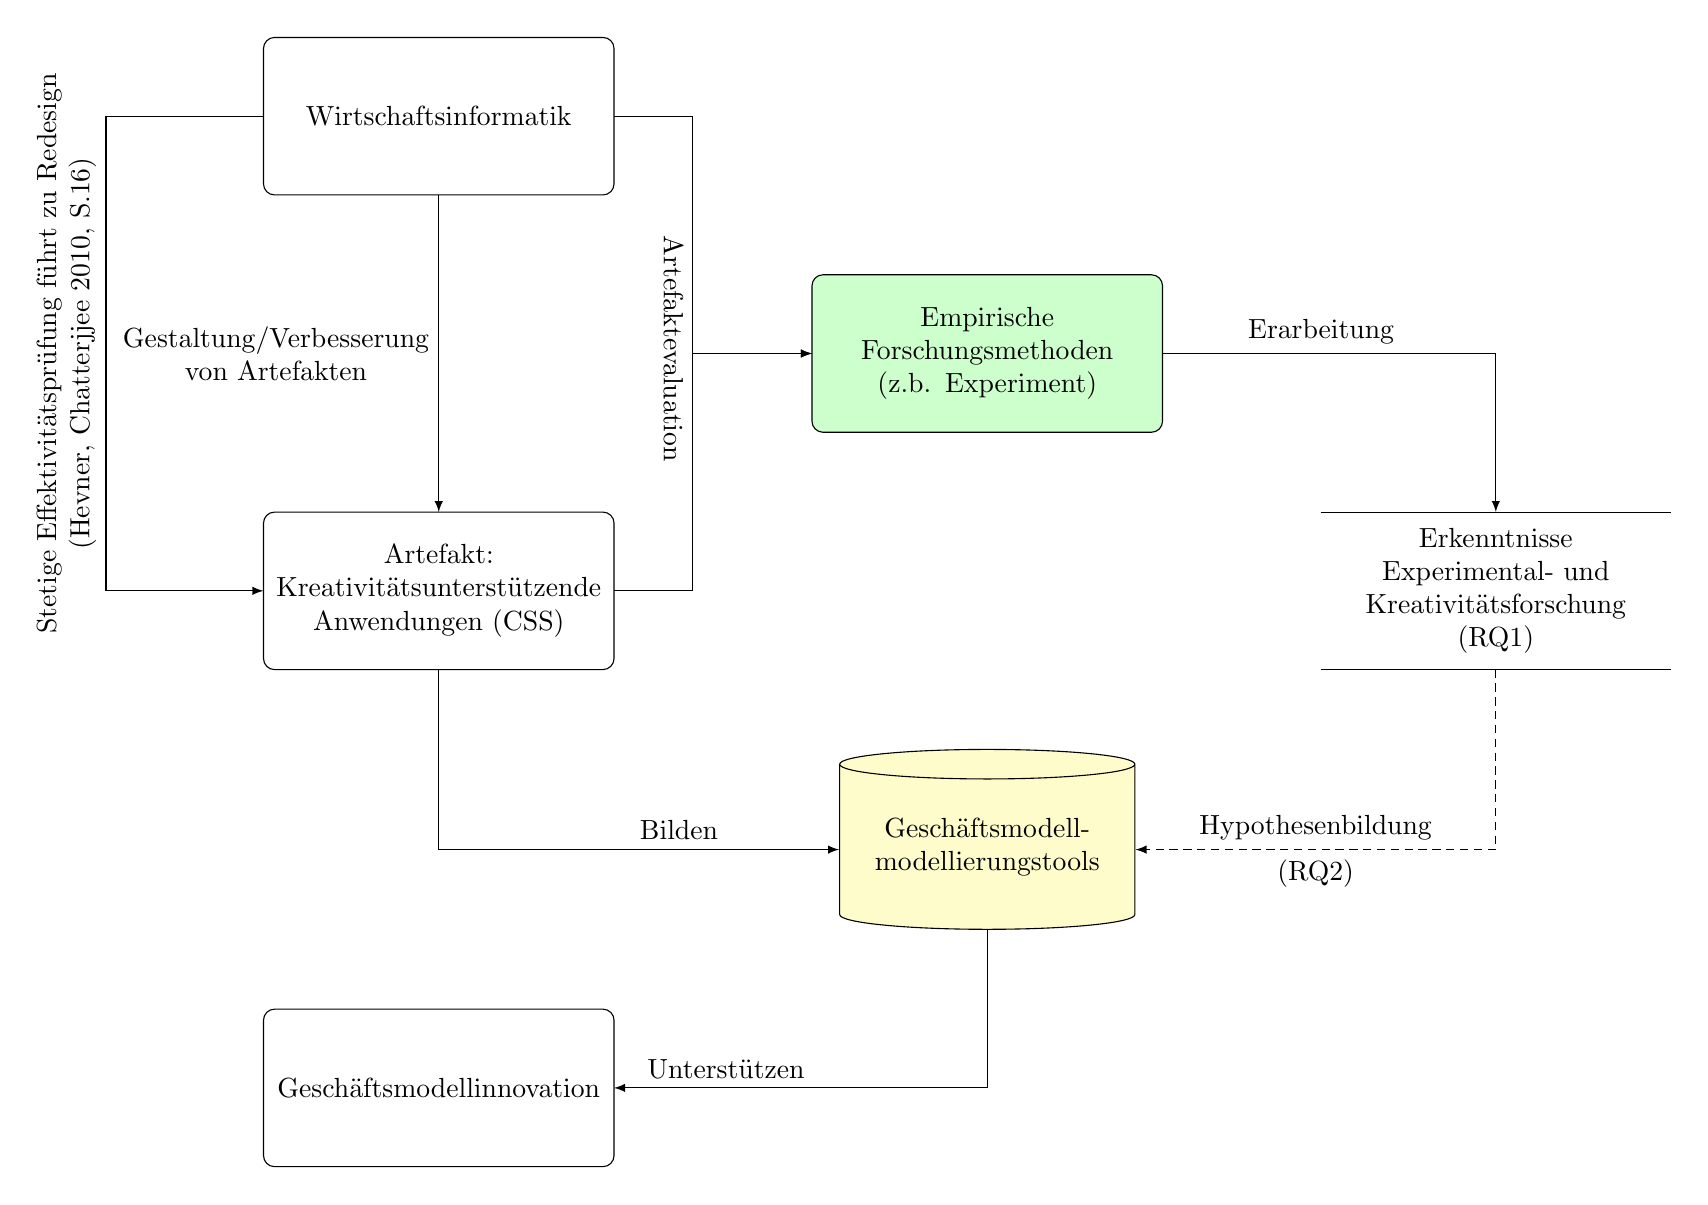
\begin{tikzpicture}%
[auto,
decision/.style={diamond, draw=blue, thick, fill=blue!20,text width=4.5em,align=flush center,inner sep=1pt},
block/.style ={ rectangle, draw, fill=white,  text centered, minimum height=15mm, text width=12em},
block_todo/.style ={ rectangle, draw, fill=white,  text centered, minimum height=15mm, text width=12em, rounded corners, outer sep=5},
block_done/.style ={ rectangle, draw, fill=white,  text centered, minimum height=15mm, text width=12em, rounded corners, outer sep=5},
block_normal/.style ={ rectangle, draw, fill=white,  text centered, minimum height=2cm, text width=12em, rounded corners, outer sep=0},
block_phantom/.style ={ block_normal, draw=none},
block_background/.style ={ rectangle,  draw, fill=none,  text centered, minimum height=15mm,fill opacity=.1, rounded corners},
output/.style ={trapezium,draw,fill=none, minimum height=10mm,  align=center, trapezium left angle=60, trapezium right angle=120, text width=50},
line_inner/.style ={draw, -latex,shorten >=0pt, shorten <=0pt},
kreis/.style ={ circle, draw, fill=white,  text centered, minimum height=15mm, text width=10em, rounded corners, outer sep=0, minimum size=.4cm},
zylinder/.style={cylinder, draw, fill=yellow!20,shape border rotate=90, text height=5, align=center, aspect=.1, text width=10em, minimum height=6.5em, minimum width=2em},
line_outer/.style ={draw, -latex,shorten >=4pt, shorten <=4pt}]
]


\matrix (table) [column sep=1.5cm,row sep=1cm, ampersand replacement=\&,  nodes in empty cells, in front of path]
{
% row 1
\node [block_normal] (11) {Wirtschaftsinformatik};  \& [1cm]
 \node [block_phantom] (12) {}; \& [.5cm]
 \node [block_phantom] (13) {}; \\
 % row 2
\node [block_phantom] (21) {};\& 
 \node [block_normal, fill=green!20] (22) {Empirische Forschungsmethoden\\(z.b. Experiment)}; \&
 \node [block_phantom] (23) {}; \\
 % row 3
\node [block_normal] (31) {Artefakt:\\Kreativit\"atsunterst\"utzende Anwendungen (CSS)};\& 
 \node [block_phantom] (32) {}; \&
 \node [block_normal, draw=none] (33) {Erkenntnisse Experimental- und Kreativit\"atsforschung\\(RQ1)}; 
  \\
 % row 4
\node [block_phantom] (41) {};\& 
 \node [zylinder] (42) {Gesch\"aftsmodell-\\modellierungstools}; \&
 \node [block_phantom] (43) {};  
   \\
 % row 5
\node [block_normal] (51) {Gesch\"aftsmodellinnovation};\& 
 \node [block_phantom] (52) {}; \&
 \node [block_phantom] (53) {}; \\
};

%%Pfeile%%%

\draw[line_inner, sloped] (11.east) -|  ++(1,0) |-   node[pos=.49, left, rotate=0, align=center, below] {Artefaktevaluation}(22.west);
\draw[line_inner] (31.east) |-  ++(1,0) |- (22.west);
\draw [line_inner] (11.south) -- node[pos=.5, left, rotate=0, align=center] {Gestaltung/Verbesserung\\von Artefakten}(31);

\draw[line_inner] (11.west) -|  ++(-2,0) |-  node[pos=.25, above, rotate=90, align=center] {Stetige Effektivit\"atspr\"ufung f\"uhrt zu Redesign \\(Hevner, Chatterjjee 2010, S.16)}(31.west);
\draw[line_inner] (22.east) -|  ++(3,0) -|  node[pos=-.4, above, rotate=0, align=center] {Erarbeitung}(33.north);
\draw[line_inner, densely dashed] (33.south) |-  ++(0,0) |-  node[pos=.75, above, rotate=0, align=center] {Hypothesenbildung} node[pos=.75, below, rotate=0, align=center] {(RQ2)}(42.east);
\draw[line_inner] (31.south) |-  ++(0,0) |-   node[pos=.8, above, rotate=0, align=center] {Bilden}(42.west);
\draw[line_inner] (42.south) |-  ++(0,0) |-   node[pos=.85, above, rotate=0, align=center] {Unterst\"utzen}(51.east);
\draw(33.south west) edge (33.south east);
\draw(33.north west) edge (33.north east);
\end{tikzpicture}%
%
}%
{%file exists=false: befinde mich im root_verzeichnis
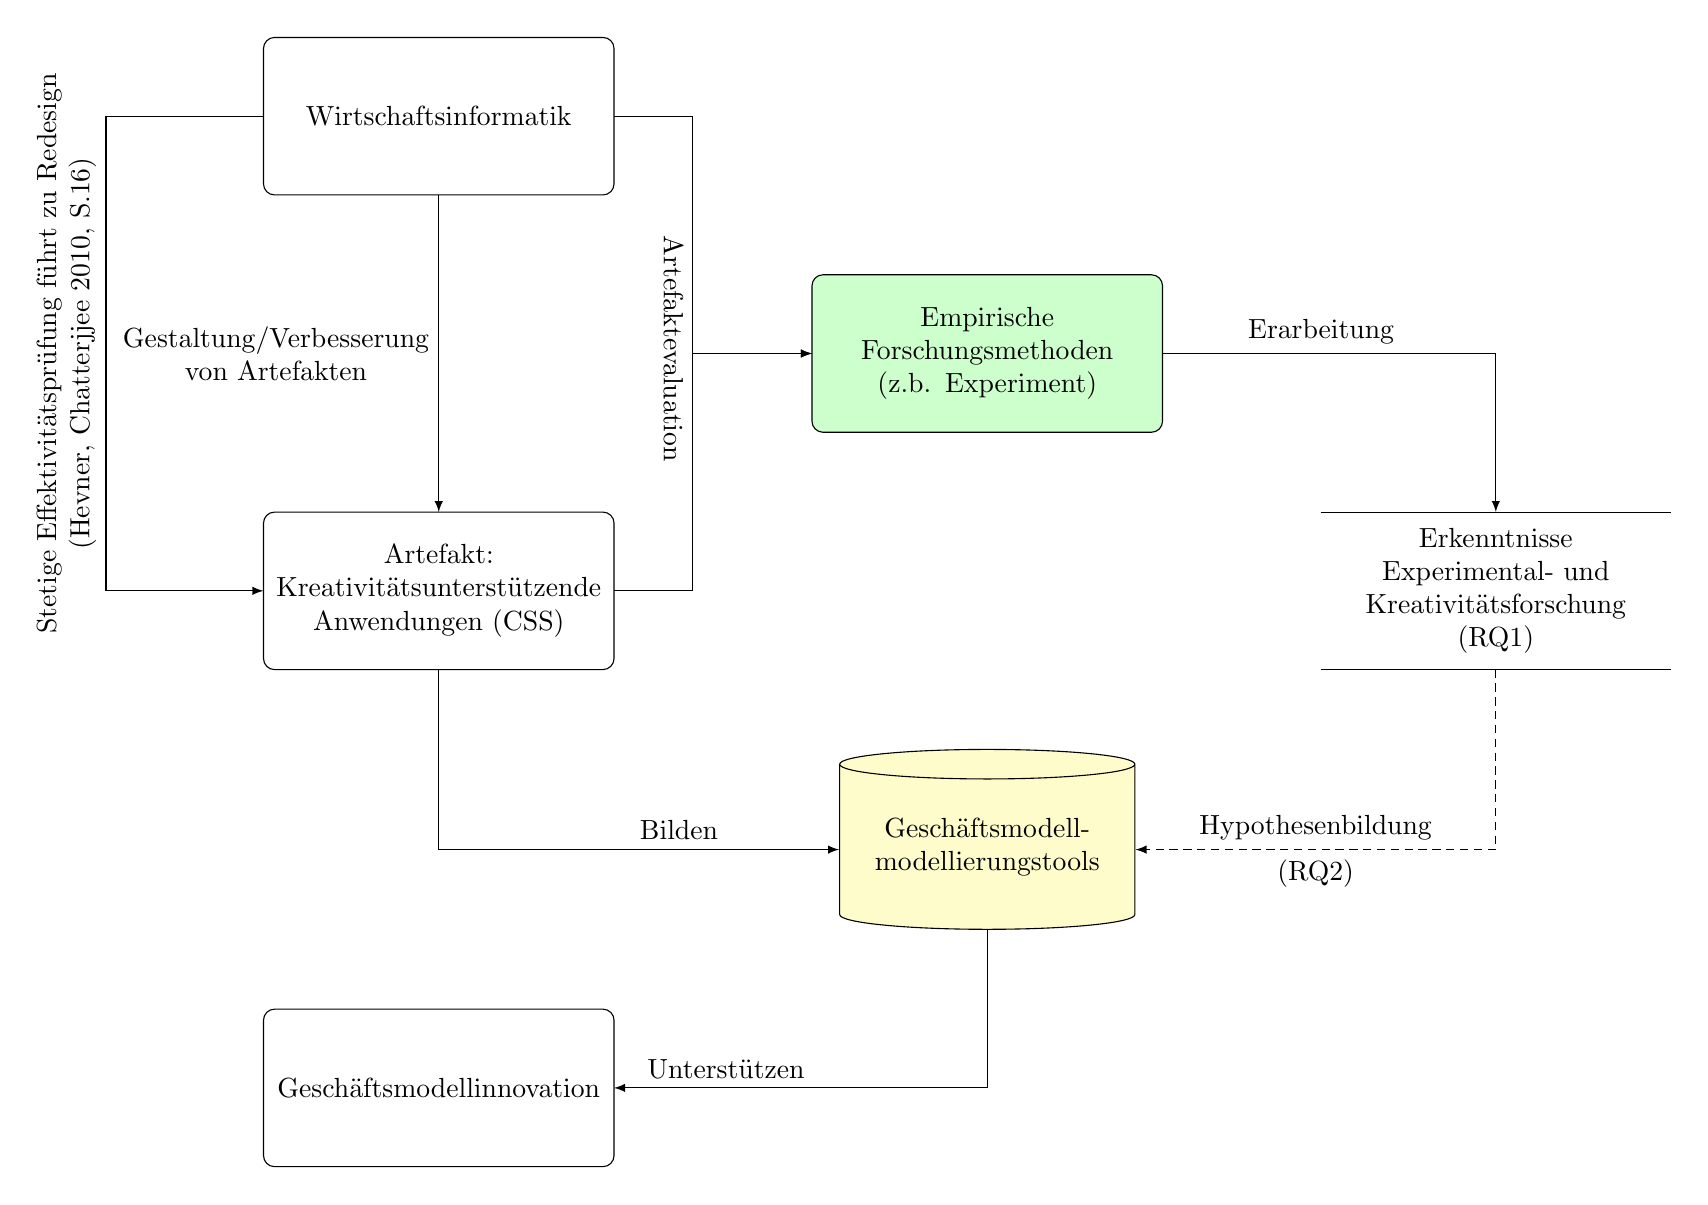
\begin{tikzpicture}%
[auto,
decision/.style={diamond, draw=blue, thick, fill=blue!20,text width=4.5em,align=flush center,inner sep=1pt},
block/.style ={ rectangle, draw, fill=white,  text centered, minimum height=15mm, text width=12em},
block_todo/.style ={ rectangle, draw, fill=white,  text centered, minimum height=15mm, text width=12em, rounded corners, outer sep=5},
block_done/.style ={ rectangle, draw, fill=white,  text centered, minimum height=15mm, text width=12em, rounded corners, outer sep=5},
block_normal/.style ={ rectangle, draw, fill=white,  text centered, minimum height=2cm, text width=12em, rounded corners, outer sep=0},
block_phantom/.style ={ block_normal, draw=none},
block_background/.style ={ rectangle,  draw, fill=none,  text centered, minimum height=15mm,fill opacity=.1, rounded corners},
output/.style ={trapezium,draw,fill=none, minimum height=10mm,  align=center, trapezium left angle=60, trapezium right angle=120, text width=50},
line_inner/.style ={draw, -latex,shorten >=0pt, shorten <=0pt},
kreis/.style ={ circle, draw, fill=white,  text centered, minimum height=15mm, text width=10em, rounded corners, outer sep=0, minimum size=.4cm},
zylinder/.style={cylinder, draw, fill=yellow!20,shape border rotate=90, text height=5, align=center, aspect=.1, text width=10em, minimum height=6.5em, minimum width=2em},
line_outer/.style ={draw, -latex,shorten >=4pt, shorten <=4pt}]
]


\matrix (table) [column sep=1.5cm,row sep=1cm, ampersand replacement=\&,  nodes in empty cells, in front of path]
{
% row 1
\node [block_normal] (11) {Wirtschaftsinformatik};  \& [1cm]
 \node [block_phantom] (12) {}; \& [.5cm]
 \node [block_phantom] (13) {}; \\
 % row 2
\node [block_phantom] (21) {};\& 
 \node [block_normal, fill=green!20] (22) {Empirische Forschungsmethoden\\(z.b. Experiment)}; \&
 \node [block_phantom] (23) {}; \\
 % row 3
\node [block_normal] (31) {Artefakt:\\Kreativit\"atsunterst\"utzende Anwendungen (CSS)};\& 
 \node [block_phantom] (32) {}; \&
 \node [block_normal, draw=none] (33) {Erkenntnisse Experimental- und Kreativit\"atsforschung\\(RQ1)}; 
  \\
 % row 4
\node [block_phantom] (41) {};\& 
 \node [zylinder] (42) {Gesch\"aftsmodell-\\modellierungstools}; \&
 \node [block_phantom] (43) {};  
   \\
 % row 5
\node [block_normal] (51) {Gesch\"aftsmodellinnovation};\& 
 \node [block_phantom] (52) {}; \&
 \node [block_phantom] (53) {}; \\
};

%%Pfeile%%%

\draw[line_inner, sloped] (11.east) -|  ++(1,0) |-   node[pos=.49, left, rotate=0, align=center, below] {Artefaktevaluation}(22.west);
\draw[line_inner] (31.east) |-  ++(1,0) |- (22.west);
\draw [line_inner] (11.south) -- node[pos=.5, left, rotate=0, align=center] {Gestaltung/Verbesserung\\von Artefakten}(31);

\draw[line_inner] (11.west) -|  ++(-2,0) |-  node[pos=.25, above, rotate=90, align=center] {Stetige Effektivit\"atspr\"ufung f\"uhrt zu Redesign \\(Hevner, Chatterjjee 2010, S.16)}(31.west);
\draw[line_inner] (22.east) -|  ++(3,0) -|  node[pos=-.4, above, rotate=0, align=center] {Erarbeitung}(33.north);
\draw[line_inner, densely dashed] (33.south) |-  ++(0,0) |-  node[pos=.75, above, rotate=0, align=center] {Hypothesenbildung} node[pos=.75, below, rotate=0, align=center] {(RQ2)}(42.east);
\draw[line_inner] (31.south) |-  ++(0,0) |-   node[pos=.8, above, rotate=0, align=center] {Bilden}(42.west);
\draw[line_inner] (42.south) |-  ++(0,0) |-   node[pos=.85, above, rotate=0, align=center] {Unterst\"utzen}(51.east);
\draw(33.south west) edge (33.south east);
\draw(33.north west) edge (33.north east);
\end{tikzpicture}%
%
}%
\end{document}%